\chapter{Technical Report}

For this project we used ASP.NET Core 2 and an SQLite3 database. This is
interacted with the Entity Framework. We also opted for a code-first approach as
 it was the most intuitive to add user authentication to.

For our user authentication system we used ASP.NET Core Identity. With this
system we were able to create a unified user database and add roles to the
registered users. These roles were then used to restrict access to specific
methods - for example guests can only get the route index and details page,
while managers and admins can create, edit and delete routes. If guests try to
access these pages they will get redirected to the login page. Normal users will
receive an $Unauthorised$ error.

\begin{figure}[ht]
  \centering
  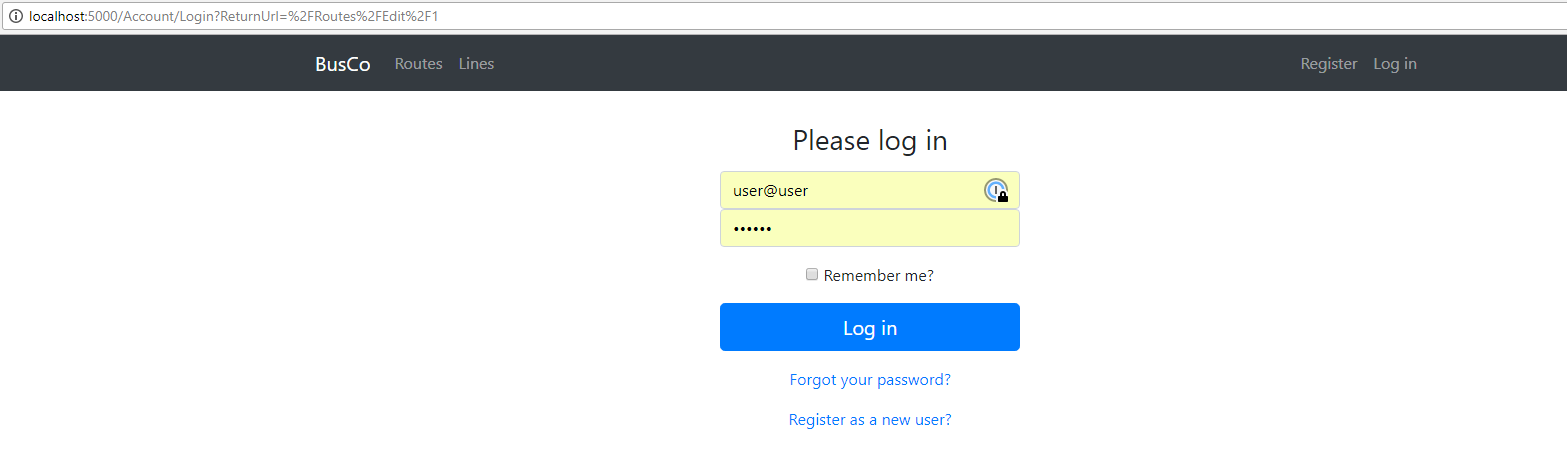
\includegraphics[width=\linewidth]{guest-unauth}
  \caption{Guest accessing $/Routes/Edit/1$, redirected to login page}
\end{figure}

\begin{figure}[ht]
  \centering
  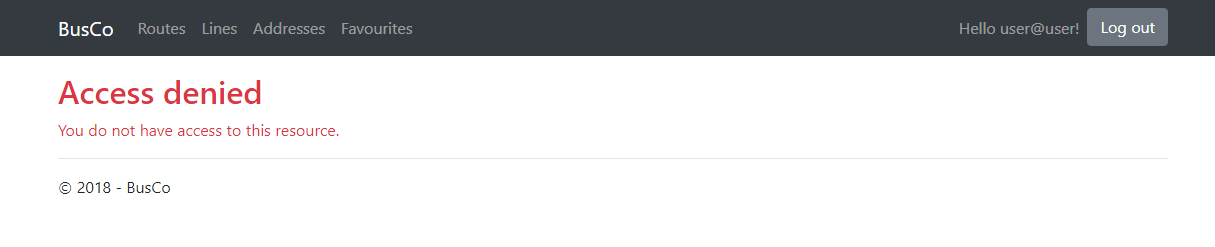
\includegraphics[width=\linewidth]{user-unauth}
  \caption{User accessing $/Routes/Edit/1$ showing unauthorised error}
\end{figure}

\begin{figure}[ht]
  \centering
  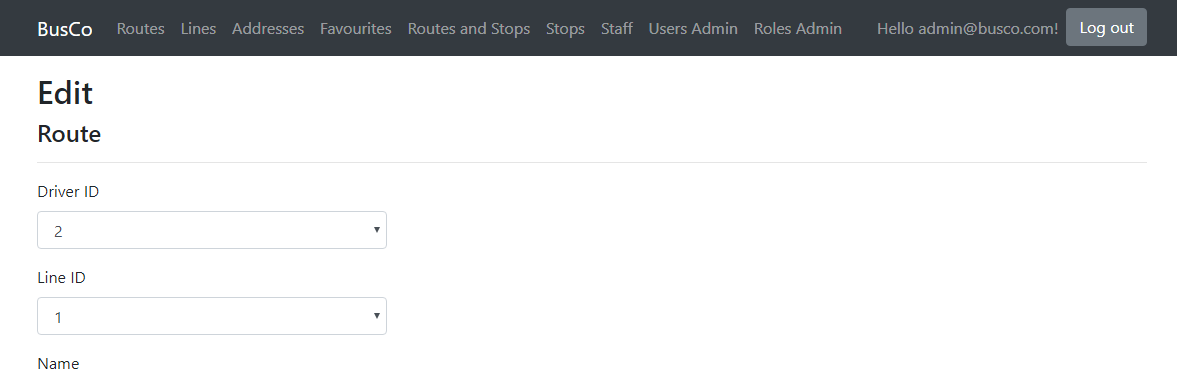
\includegraphics[width=\linewidth]{manager-unauth}
  \caption{Manager accessing $/Routes/Edit/1$ and getting the edit page displayed}
\end{figure}

